\setchapterstyle{kao}
%\setchapterpreamble[u]{\margintoc}
\chapter{Embedding sentences with large transformer models}
%Training sentence embedding models using discriminative objective}
\labch{1B}

\cleanchapterquote{Give orange me give eat orange me eat orange give me eat orange give me you.}{Nim Chimpsky}{Male chimpanzee, 1979}

The previous sections discussed the importance of neural model structure in composing sentence representations. Along with the architecture of the sentence encoder, other parameters may strongly influence the quality of the embeddings. In particular, the last few years have seen a race to increase the number of parameters, hidden size, or size of pre-training data. As already observed in \refch{arithmetics} or \refsec{survey:downstream}, scaling models is an established method for improving downstream results\sidenote{The effect of scaling is considered so obvious that it was used as the primary reason to reject RoBERTa  paper \parencite{liu_2019} from ICLR 2020. As expressed by the Program Chairs: "most of the findings are obvious (careful tuning helps, more data helps)". \url{https://openreview.net/forum?id=SyxS0T4tvS}}.

The following sections aims to train and evaluate sentence embedding models at scale. \refch{1B} presents an attempt to train state-of-the-art sentence embedding models on a very large corpus. \refch{generative} propose to train the first large generative pre-trained model in French. Finally, \refch{structure-scale} proposes to train structured models at scale.

\section{Training language models at scale}
\labsec{scale}

% we review the challenges and benefits of large models. \refsec{1B}
"Just add more layers" seems to be the new mantra for efficient deep learning. As opposed to deriving complex architectures from linguistic insights, it might be easier to focus on efficient and parallelizable networks, which are easy to scale. As illustrated in \reffig{large-models}, the number of parameters for large language models follows what we may compare with the Moore's Law.

\begin{figure}[htb!]
	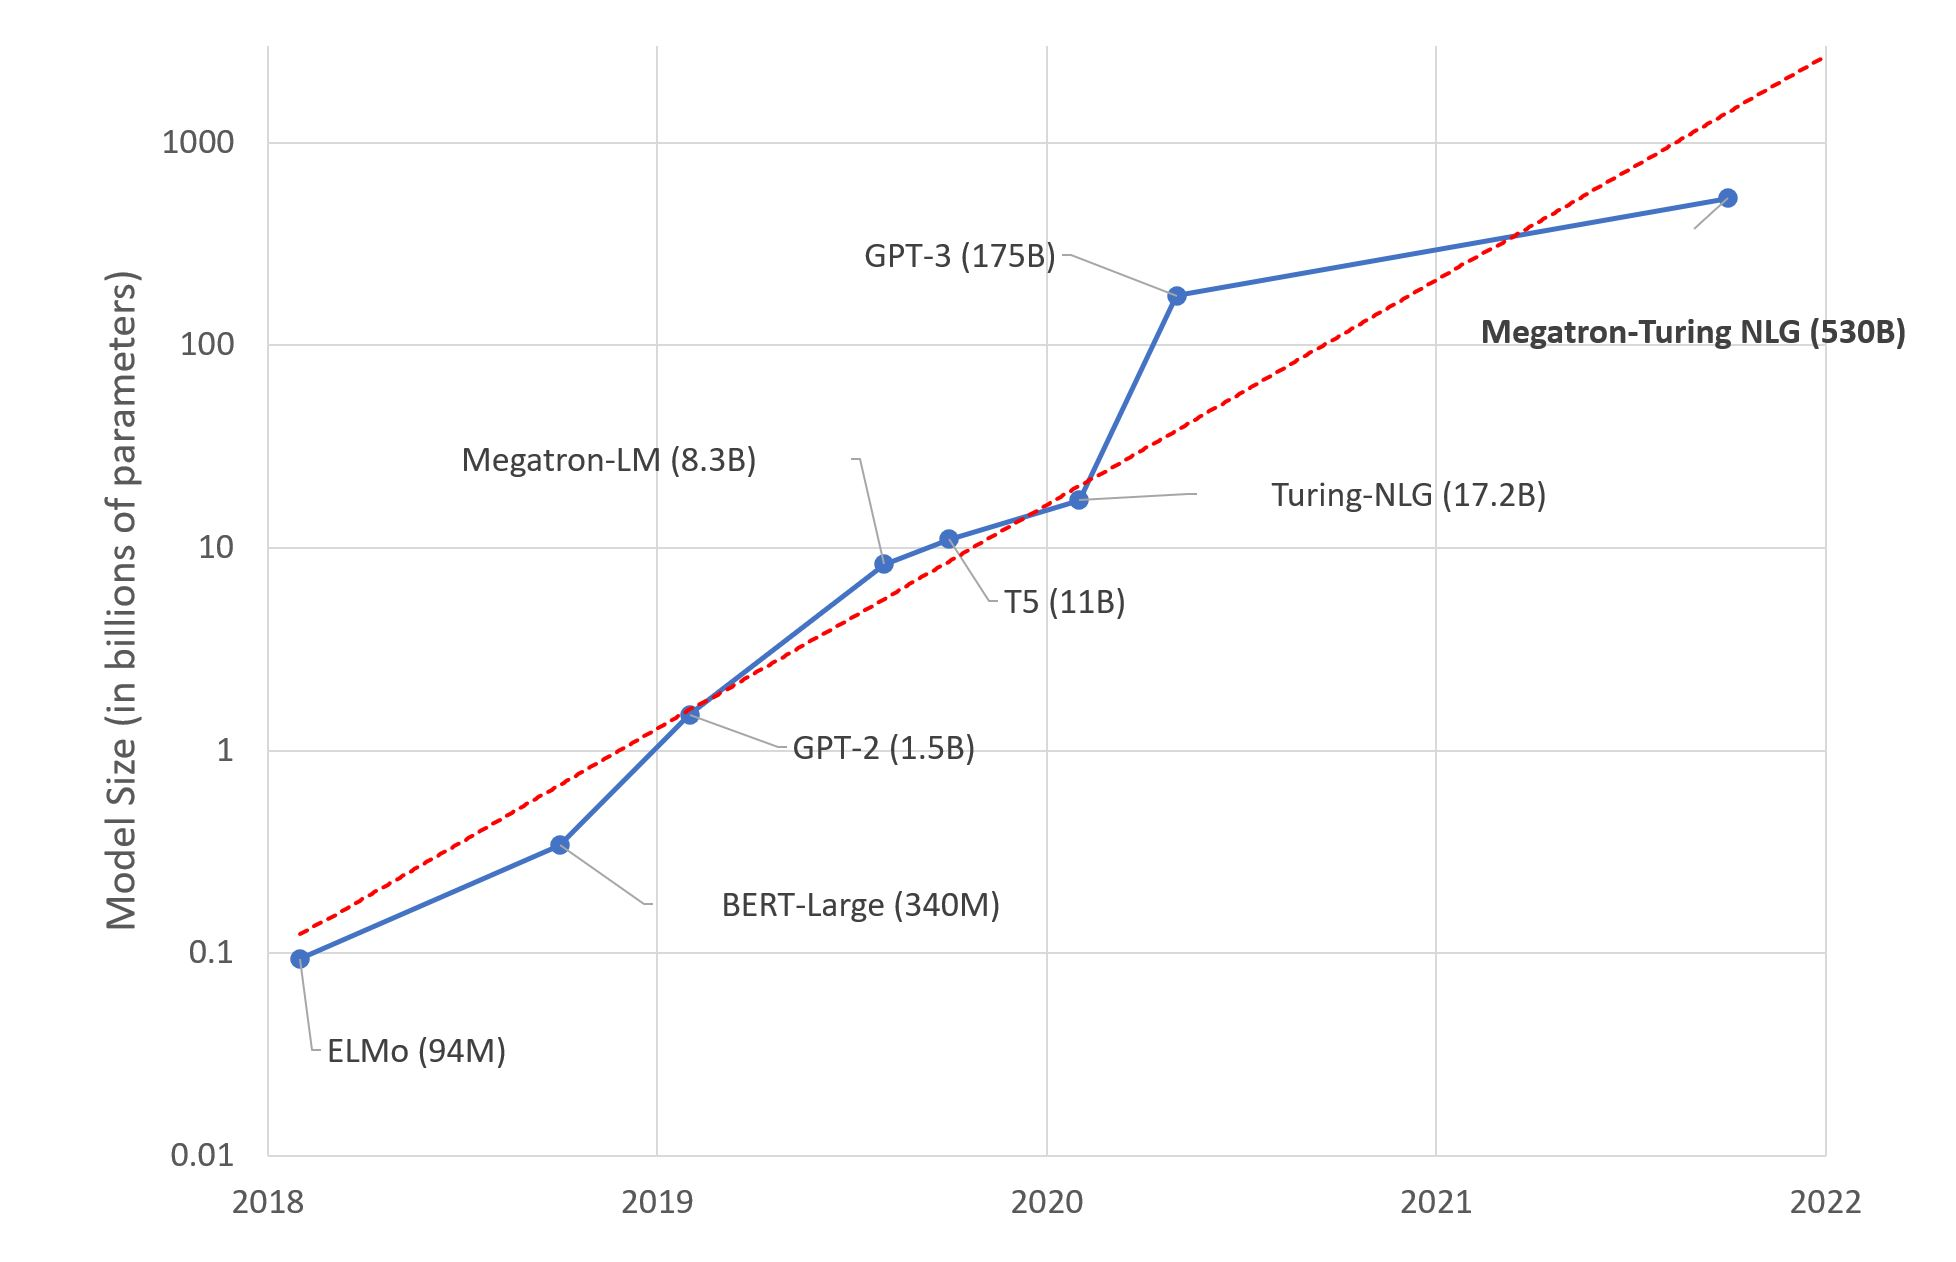
\includegraphics[width=\textwidth]{images/model-size-graph.jpeg}
	\caption[Large models number of parameters]{Evolution of the number of parameters for large language models. The figure is extracted from Microsoft \href{https://www.microsoft.com/en-us/research/blog/using-deepspeed-and-megatron-to-train-megatron-turing-nlg-530b-the-worlds-largest-and-most-powerful-generative-language-model/}{blog post}.}
	\labfig{large-models}
\end{figure}

Language models also seem to support the adage, "the bigger, the better". On the GLUE benchmark for example, the base version of \textsc{Bert} with 100M parameters achieves an average score of 79.6 while the large version with 340M parameters achieves 82.1. Besides the number of parameters, the architecture, the training procedure, as well as the training data remain unchanged. The training at scale seems also to leverage some particular behaviors, mediated by some threshold effects. For example \textcite{brown_20} compare generative pre-trained models with distinct sizes on few-shot learning settings. While the smallest model with 1.3B parameters do not show any abilities on the task, the largest model with 175B parameters show surprisingly good generalization performances with a very limited number of training examples.

Even though the effect of scaling is no longer a surprise, training large models continues to be a challenging exercise. Training large models poses many challenges for optimization \parencite{you_20}, infrastructure \parencite{shoeybi_19, narayanan_21} or data collection \parencite{OrtizSuarezSagotRomary2019}. 

% \section{Train a sentence embedding model with 1 billion training pairs}
% \labsec{1B}

% In this section, we review the challenges and benefits of large models.
This section relates the development of state-of-the-art sentence embedding models as part of the project \textit{Train the Best Sentence Embedding Model Ever with 1B Training Pairs}\footnote{\url{https://discuss.huggingface.co/t/train-the-best-sentence-embedding-model-ever-with-1b-training-pairs/7354}}. This project took place during the \textit{Community week using JAX/Flax for NLP \& CV}\footnote{\url{https://discuss.huggingface.co/t/open-to-the-community-community-week-using-jax-flax-for-nlp-cv/7104}}, organized by Hugging Face. Our project was among the winners of the competition and received an honorable mention. As part of this project, I contributed actively to the construction of the dataset, the training and documentation of the sentence embedding models. The following section is adapted from a post I published in Hugging Face blog\sidenote{\url{https://huggingface.co/blog/1b-sentence-embeddings}}.

\section{Training framework}

We use a contrastive training objective and collect sentence pairs $(a_i, p_i)$ that are somehow semantically related. The effective construction of the dataset is detailed in \refsec{1B:dataset}. We train the model to map pairs $(a_i , p_i)$ to close vectors while assigning unmatched pairs $(a_i , p_j)_{i \neq j}$ to distant vectors in the embedding space. This training method closely relates quick-thoughts (presented in \refsec{training}), contrastive unsupervised representation learning \parencite{saunshi_19}, training with in-batch negatives \parencite{carlsson_21}, InfoNCE \parencite{oord_18} or NTXentLoss \parencite{sohn_16}.

We illustrate the training objective in \reffig{contrastive}. Intuitively, the model should assign high similarity to the sentences « How many people live in Berlin? » and « Around 3.5 million people live in Berlin » and low similarity to other negative answers such as « The capital of France is Paris ».

\begin{figure}[htb!]
	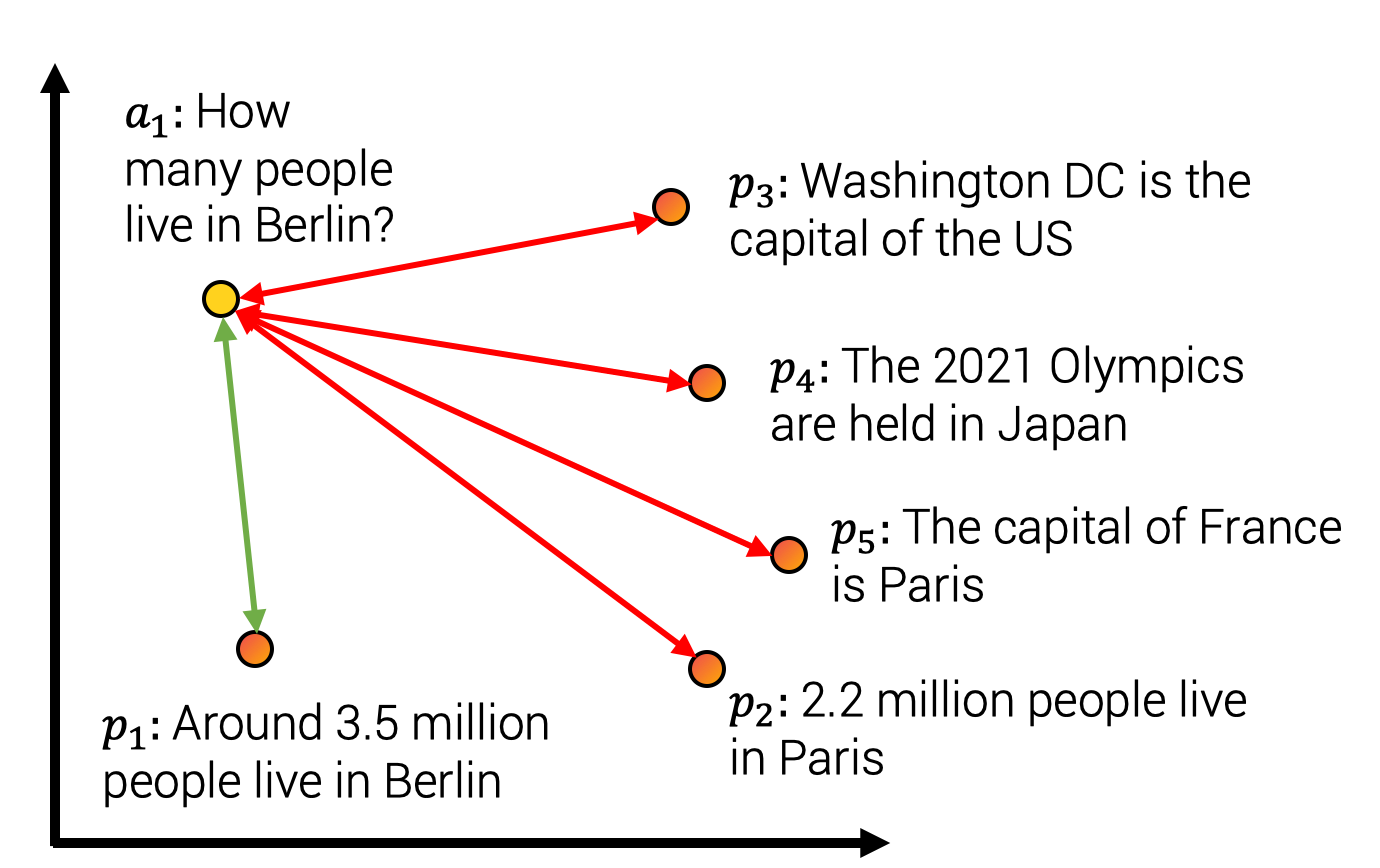
\includegraphics[width=10cm]{images/contrastive_1.png}
	\caption[Contrastive learning]{Illustration of the contrastive learning setup. The model is trained to associate an anchor sentence with another one that is semantically related. The notion of semantic relation depends on the nature of the pair. Our example aims to link the correct answer to a given question. City capitals are the subject of all these sentences, but only one is the correct answer.}
	\labfig{contrastive}
\end{figure}

As in other contrastive methods detailed in \refsec{training:self-supervised}, we build negative pairs by considering other samples from the batch. Given a batch of $n$ training samples, the model optimises the following loss function:

\begin{equation}
    \mathcal{L} = -\frac{1}{n}\sum_{i=1}^n\frac{e^{c(a_i, p_i)}}{\sum_j e^{c(a_i, p_j)}}    
\end{equation}

Where $c$ is a \textit{critic function}, which measures the distance between two sentence embeddings $(a, p)$\sidenote{A set of possible critics is presented in \cite{tschannen_19}. Most used functions are either the cosine similarity or the dot product operator. The cosine similarity have the nice advantage to present the highest similarity to itself since $cos(a, a) =1$. While with the dot-product other vectors can have higher similarities: $dot(a, a) < dot (a, b)$.}.

%We illustrate the training objective in \reffig{contrastive-2}.

% \begin{figure}[htb!]
% 	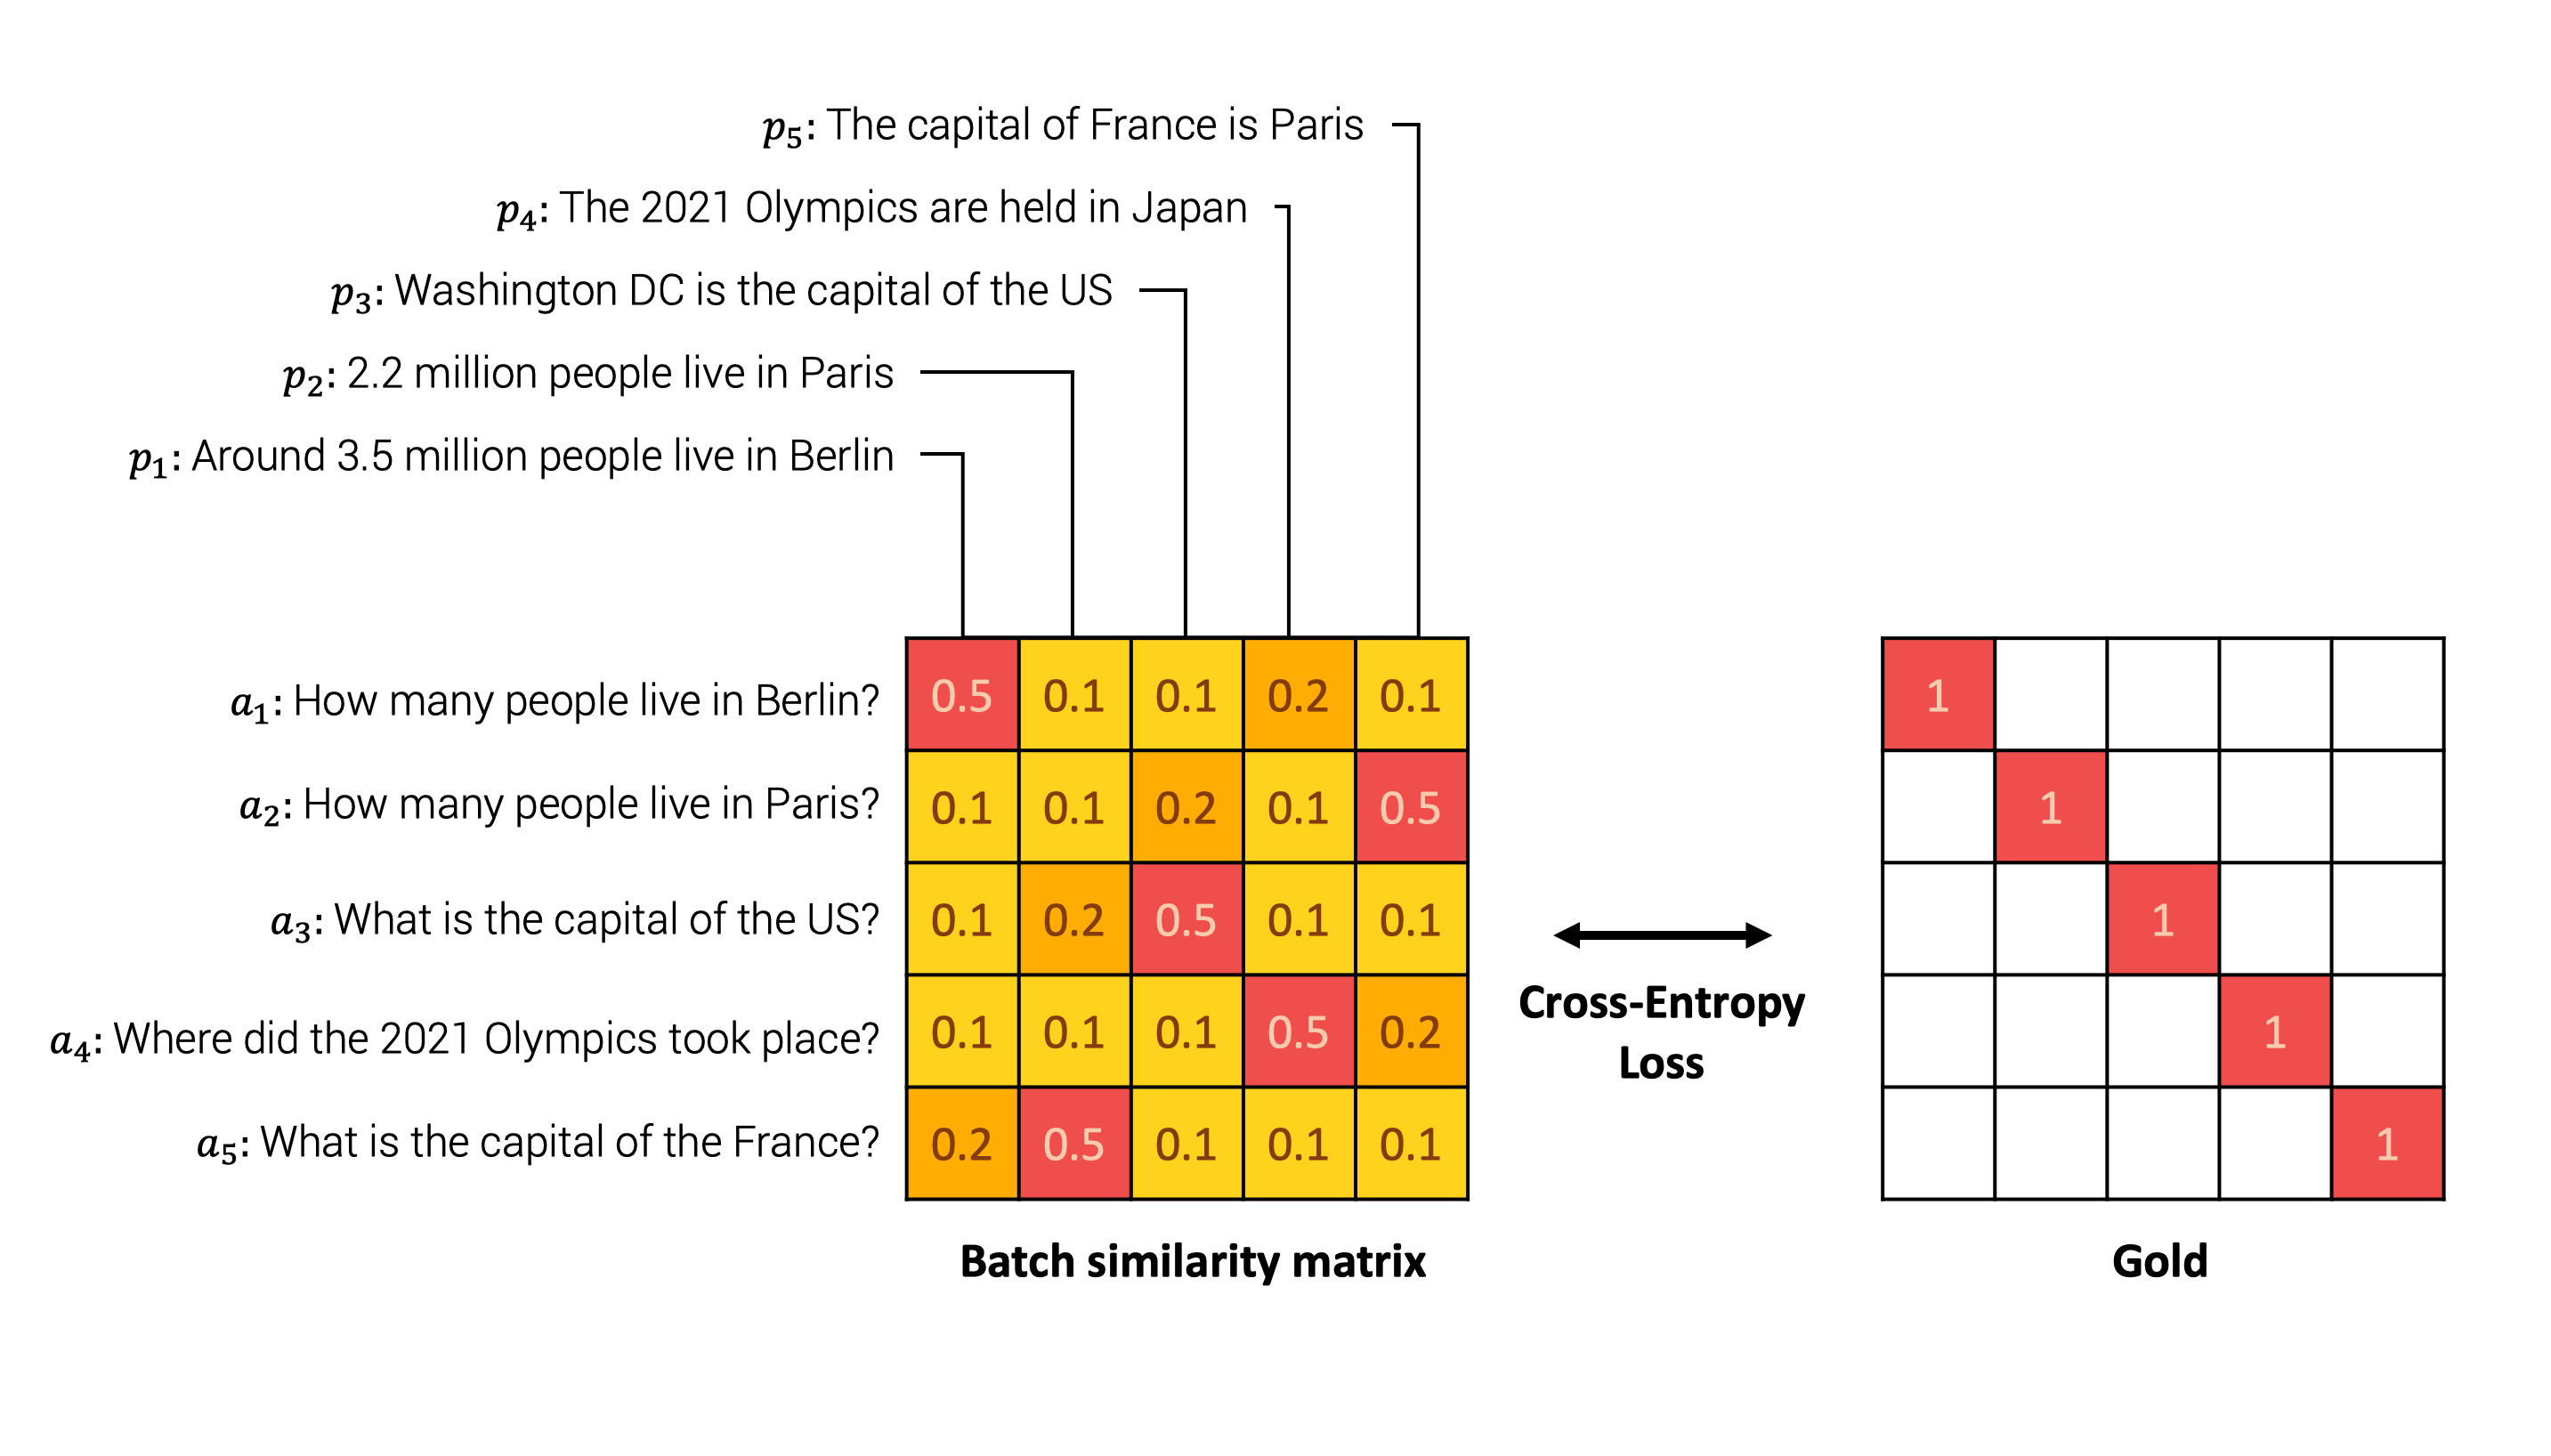
\includegraphics[width=10cm]{images/contrastive_2.png}
% 	\caption[Contrastive learning]{Illustration of the contrastive learning objective.}
% 	\labfig{contrastive-2}
% \end{figure}

\section{Construction of the dataset}
\labsec{1B:dataset}

We constitute a dataset with sentence pairs $(a_i, p_i)$ such that sentences from the pair have a close meaning. We considered pairs such as (query, answer-passage), (question, duplicate\_question), (paper title, cited paper title). We aggregated many existing datasets enumerated in \reftab{tab:1B:dataset}. 

The majority of the dataset is build out of Reddit comments. Reddit website aggregates news, and lets users post links and discuss trought threads. We use scripts from PolyAI\sidenote{\url{https://github.com/PolyAI-LDN/conversational-datasets/tree/master/reddit}} to generate tuples given the first comment for each response. We filter out samples with more than 128 characters, or fewer than 9 characters. I personally took care of this data collection operation.

\begin{table*}[!htb]
\centering
\small
\begin{tabularx}{16cm}{@{}lp{4.5cm}Y@{} }
\toprule
\textbf{Dataset} & \textbf{Reference} & \textbf{Number of training pairs} \\
\midrule
\midrule 
\href{https://github.com/PolyAI-LDN/conversational-datasets/tree/master/reddit}{Reddit Comments} (2015-2018) & \textcite{henderson_19} & \num{726484430} \\
\href{https://github.com/allenai/s2orc}{S2ORC} citation pairs (abstracts) & \textcite{lo_20} & \num{116288806} \\
\href{https://github.com/afader/oqa#wikianswers-corpus}{WikiAnswers} duplicate question pairs & \textcite{fader_14} & \num{77427422} \\
\href{https://github.com/facebookresearch/PAQ}{PAQ} (question, answer) pairs & \textcite{lewis_21} & \num{64371441} \\
\href{https://github.com/allenai/s2orc}{S2ORC} citation pairs (titles) & \textcite{lo_20} & \num{52603982} \\
\href{https://github.com/allenai/s2orc}{S2ORC} (title, abstract) & \textcite{lo_20} & \num{41769185} \\
\href{https://huggingface.co/datasets/flax-sentence-embeddings/stackexchange_xml}{Stack Exchange} (title, body) pairs & - & \num{25316456} \\
\href{https://microsoft.github.io/msmarco/}{MS MARCO} triplets & \textcite{craswell_21} & \num{9144553} \\
\href{https://github.com/allenai/gooaq}{GOOAQ} & \textcite{khashabi_21} & \num{3012496} \\
\href{https://www.kaggle.com/soumikrakshit/yahoo-answers-dataset}{Yahoo Answers} (title, answer) & \textcite{zhang_15} & \num{1198260} \\
\href{https://huggingface.co/datasets/code_search_net}{Code Search} & - & \num{1151414} \\
\href{https://cocodataset.org/#home}{COCO} image captions & \textcite{lin_14} & \num{828395} \\
\href{https://github.com/allenai/specter}{SPECTER} citation triplets & \textcite{cohan_20} & \num{684100} \\
\href{https://www.kaggle.com/soumikrakshit/yahoo-answers-dataset}{Yahoo Answers} (question, answer) & \textcite{zhang_15} & \num{681164} \\
\href{https://www.kaggle.com/soumikrakshit/yahoo-answers-dataset}{Yahoo Answers} (title, question) & \textcite{zhang_15} & \num{659896} \\
\href{https://huggingface.co/datasets/search_qa}{SearchQA} & \textcite{dunn_17} & \num{582261} \\
\href{https://huggingface.co/datasets/eli5}{Eli5} & \textcite{fan_19} & \num{325475} \\
\href{https://shannon.cs.illinois.edu/DenotationGraph/}{Flickr 30k} & \textcite{young_14} & \num{317695} \\
\href{https://huggingface.co/datasets/flax-sentence-embeddings/stackexchange_xml}{Stack Exchange} duplicate questions (titles) & - & \num{304525} \\
AllNLI (\href{https://nlp.stanford.edu/projects/snli/}{SNLI} and \href{https://cims.nyu.edu/~sbowman/multinli/}{MultiNLI}) & \textcite{bowman_15, williams_18b} & \num{277230} \\
\href{https://huggingface.co/datasets/flax-sentence-embeddings/stackexchange_xml}{Stack Exchange} duplicate questions (bodies) & - & \num{250519} \\
\href{https://huggingface.co/datasets/flax-sentence-embeddings/stackexchange_xml}{Stack Exchange} duplicate questions (titles and bodies) & - & \num{250460} \\
\href{https://github.com/google-research-datasets/sentence-compression}{Sentence Compression} & \textcite{filippova_13} & \num{180000} \\
\href{https://github.com/pvl/wikihow_pairs_dataset}{Wikihow} & \textcite{koupaee_18} & \num{128542} \\
\href{https://github.com/chridey/altlex/}{Altlex} & \textcite{hidey_16} & \num{112696} \\
\href{https://quoradata.quora.com/First-Quora-Dataset-Release-Question-Pairs}{Quora Question Triplets} & - & \num{103663} \\
\href{https://cs.pomona.edu/~dkauchak/simplification/}{Simple Wikipedia} & \textcite{coster_11} & \num{102225} \\
\href{https://ai.google.com/research/NaturalQuestions}{Natural Questions (NQ)} & \textcite{kwiatkowski_19} & \num{100231} \\
\href{https://rajpurkar.github.io/SQuAD-explorer/}{SQuAD2.0} & \textcite{drajpurkar_18} & \num{87599} \\
\href{https://huggingface.co/datasets/trivia_qa}{TriviaQA} & - & \num{73346} \\
\midrule
\textbf{Total} & & \textbf{\num{1124818467}} \\
\bottomrule
\end{tabularx}
\caption{Sub-datasets concatenated}
\labtab{tab:1B:dataset}
\end{table*}

\section{Training}

We fine-tuned existing pre-trained models with our contrastive learning objective. As a sentence representation, we took the mean of every token hidden state from transformer models. We applied 500 warm-up steps and use a batch size of 64 if not explicitly specified otherwise. We created 20 general-purpose Sentence Transformers models such as Mini-LM \parencite{wang_20a}, RoBERTa \parencite{liu_2019}, DistilBERT \parencite{sanh_19} and MPNet \parencite{song_20}\sidenote{All models created during the challenge are available as open source contributions in our HuggingFace repository \url{https://huggingface.co/flax-sentence-embeddings}.}. 

\begin{figure}[htb!]
	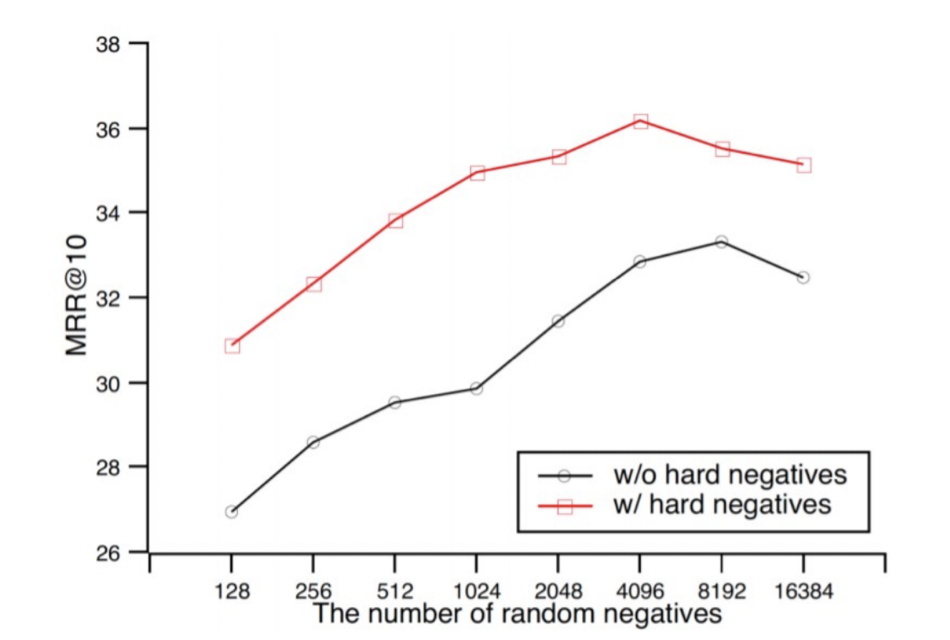
\includegraphics[width=10cm]{images/batch-size.png}
	\caption[Batch size]{Influence from the batch size and selection of hard negative on downstream evaluation. The figure is extracted from \textcite{qu_21}.}
	\labfig{batch-size}
\end{figure}

When building models, the selection of pairs forming a batch is crucial. Here we examine the batch characteristics and their impact on the embeddings.

\paragraph{Batch size} The quick-thoughts method detailed in \refsec{training:self-supervised} uses a rather important batch size of 400. In fact, studies show that the more large the batch, the better the performances  \parencite{chen_20a, qu_21}. This trend is illustrated \reffig{batch-size} extracted from \textcite{qu_21}. Yet, too important batch size may decrease the results (the same asymptotic phenomenon is observed in \textcite{chen_20a}).  We benefited from efficient hardware infrastructure to run the project: 7 TPUs v3-8, as well as guidance from Google’s Flax, JAX, and Cloud team members about efficient deep learning frameworks. We use the largest batch size that our hardware could fit, in our case, 64.

\paragraph{Hard Negatives}  We may build batches by uniformly selecting samples from the training data. As detailed in \textcite{robinson_21} or \textcite{qu_21}, the selection of "good negative examples" yet significantly impacts the training process. The impact of hard negative is illustrated in \reffig{batch-size}.
Hard negative examples should not correspond to the anchor point but still be difficult to distinguish from the correct associations. 
% Hard negatives are sample $p_j$, which are hard to distinguish from $p_i$. 
In our example, it could be the pairs « What is the capital of France? » and « What is the capital of the US? » which have a close semantic content and requires precisely understanding the full sentence to be answered correctly. On the contrary, the samples « What is the capital of France? » and «How many Star Wars movies is there?» are less difficult to distinguish since they do not refer to the same topic.

\paragraph{Cross dataset batches} In our case, the dataset is a concatenation of several sub-datasets (\reftab{tab:1B:dataset}). Each sub-dataset is build on distinct topics, domains or semantic relation in the pairs. We want to avoid the case where our model learn disjoint embeddings spaces for each sub-dataset. On the other hand, mixing all sub-datasets in the same batch may deteriorate the hard negatives proportion as samples issue from two sub-datasets should be easy to differentiate. To address both requirements, we build batches from the mix of only two sub-datasets. We aim therefore to learn a global structure between topics and not only a local structure within a topic while not too much deteriorating the proportion of hard negatives.

\section{Evaluation}

As detailed in \refsec{survey:downstream}, sentence embeddings are traditionally evaluated on the SentEval benchmark. However, as detailed in the same section, the benchmark suffers from practical limitations or biases. For this project, we therefore used a dedicated benchmark to compare our models\sidenote{\url{https://github.com/nreimers/se-benchmark}}. The benchmark aggregates multiple general-purpose sentence evaluation tasks. The tasks, detailed below, are formatted as binary classification, clustering, reranking, retrieval and semantic textual similarity (STS). All tasks use the embedding as features and compare them using similarity metrics. Most importantly, they do not require the training of additional classifiers.

\paragraph{Binary classification} aims at predicting a binary relation between a pair of sentences. It computes the cosine similarity between every pair of sentences. We then classify the sentence pairs by comparing their similarity score to a given threshold. We set the threshold to ensure the best score on the development set. The task includes identifying paraphrases from LanguageNet, a collection of sentences from Twitter linked through shared URLs \sidenote{\url{https://languagenet.github.io/}} or the SemEval-2015 Task 1 \sidenote{\url{https://alt.qcri.org/semeval2015/task1/}}, and identifying duplicated questions\sidenote{\url{https://www.aclweb.org/anthology/D18-1131/}}. We measure the performances using accuracy.

\paragraph{Clustering} organizes documents into semantically consistent groups. We use data from web forums and news groups, which organizes posts given their topics. We use embeddings as features for K-Means clustering and evaluation using the V-measure\sidenote{\url{https://scikit-learn.org/stable/modules/generated/sklearn.metrics.v_measure_score.html}}. The clustering task includes the 20Newsgroups\sidenote{\url{https://scikit-learn.org/0.19/datasets/twenty_newsgroups.html}}, and clustering threads from Stackexchanges and Reddit. 

\paragraph{Retrieval} aims at retrieving documents from a corpus which match the semantic content of a given query. We use datasets scraped from web forums and question-answering websites. On such platforms, experienced users can flag a question as a duplicate if it has already been answered elsewhere. We use these annotations to associate a given question to a list (of variable size) of semantically equivalent formulations. Given the embedding of a query, we compute the cosine similarity with other questions from the dataset and retrieve the top-$k$ most similar ones (by default, we use $k=10$). We then compare our predicted list with the related questions using the Mean Reciprocal Rank (MRR) or Mean average precision (MAP). The task includes CQADupStack, a dataset with duplicate question information from StackExchange subforums\sidenote{\url{http://nlp.cis.unimelb.edu.au/resources/cqadupstack/}} and the Quora Question Pairs dataset\sidenote{\url{https://quoradata.quora.com/First-Quora-Dataset-Release-Question-Pairs}}.

\paragraph{Reranking} ranks a list of document given their semantic similarity with a given query. In our setup, the task takes a query and a fixed-length list of documents as input. Each document in the list is either "similar" or "non-similar" to the query. We compute the cosine similarity between the embedding of the query and each document and sorts them in decreasing order. We then compare the sorted list with the document ordered as similar first followed by non-similar. We also use MRR@10 and MAP to measure the quality of the ranking. As in the retrieval task, data are collected from web forums but with a different format and labelling process. We use a collection of questions taken from AskUbuntu.com 2014 corpus dump\sidenote{\url{https://github.com/taolei87/askubuntu}}, SciDocs, which consider scientific papers as related based on their inter citations \sidenote{\url{https://allenai.org/data/scidocs}} and the Stack Overflow Duplicate Questions Task\sidenote{\url{https://www.microsoft.com/en-us/research/uploads/prod/2019/03/nl4se18LinkSO.pdf}}.

\paragraph{Semantic Textual Similarity (STS)} measures the semantic similarity between two sentences. Annotators assign a similarity score for pair of sentences, ranging from 0 for no overlap to 5 for meaning equivalence. The annotation doesn't require formal linguistic expertise. Performance compare the correlation between predicted scores and human judgments with Pearson correlation. The predicted scores directly measure the cosine similarity between two sentence pairs and compare it with gold human annotations (scaled between 0 and 1). The evaluation datasets include the STSBenchmark\sidenote{\url{http://ixa2.si.ehu.eus/stswiki/index.php/STSbenchmark}} which includes datasets used for the SemEval task from 2012 to 2017, the SICK-R task (already introduced in \refsec{sts}) and BIOSSES \sidenote{\url{https://tabilab.cmpe.boun.edu.tr/BIOSSES/DataSet.html}} which comprises 100 sentence pairs from the biomedical field.

% \begin{table}[ht!]
% \begin{center}
% \small
% {\renewcommand{\arraystretch}{1.25}
% \begin{tabular}{|c|p{0.88\linewidth}|}
% \hline
% \multirow{4}{*}{5}& \emph{The two sentences are completely equivalent, as they mean the same thing.}\\
% \cline{2-2}
% & The bird is bathing in the sink. \newline Birdie is washing itself in the water basin. \\
% \hline
% \multirow{4}{*}{4}  & \emph{The two sentences are mostly equivalent, but some {\it unimportant} details differ.}\\
% \cline{2-2}
% & Two boys on a couch are playing video games. \newline Two boys are playing a video game. \\
% \hline
% \multirow{4}{*}{3} & \emph{The two sentences are roughly equivalent, but some {\it important information} differs/missing.}\\
% \cline{2-2}
% & John said he is considered a witness but not a suspect. \newline ``He is not a suspect anymore.'' John said.  \\
% \hline
% \multirow{4}{*}{2} & \emph{The two sentences are not equivalent, but share some details.}\\
% \cline{2-2}
% & They flew out of the nest in groups. \newline They flew into the nest together. \\
% \hline
% \multirow{4}{*}{1} & \emph{The two sentences are not equivalent, but are on the same topic.}\\
% \cline{2-2}
% & The woman is playing the violin. \newline The young lady enjoys listening to the guitar. \\
% \hline
% \multirow{4}{*}{0} & \emph{The two sentences are completely dissimilar.}\\
% \cline{2-2}
% & The black dog is running through the snow. \newline A race car driver is driving his car through the mud. \\
% \hline
% \end{tabular}
% }
% \end{center}
% \caption{Similarity scores with explanations and English examples. The table is exctracted from \textcite{cer_17}.}
% \label{fig:annotationcore}
% \end{table}

We evaluate our models on the benchmark and report the mean score over all task on \reftab{1B-results}. The challenge was limited in time and we could not extensively trained all models with the same number of steps. We report the number of training steps. Yet, models may therefore not be directly compared.

\begin{table}[!htb]
\centering
\small
\begin{tabularx}{\textwidth}{@{}lYYY@{} }
\toprule
\textbf{Models} & \textbf{\# Training steps} ($\times 10^3$) & \textbf{Mean score} \\
\midrule
\midrule 
RoBERTa-large & 400 & 70.22 \\
MPNet-base & 440 & 70.01 \\ % & \num{1200} 
Mini-LM (12 layers, batch size 128) & 540 & 68.83 \\ % -L12-H384-uncased-batch128
RoBERTa-distill-base & 920 & 68.72 \\
Mini-LM (6 layers, batch size 128) & \num{1000} & 68.05 \\ % -L6-H384-uncased-batch128
% \midrule
% mpnet-base & - & 67.97 \\
% distil-\textsc{RoBERTa}-base & - & 66.27 \\
% TinyBERT-L6 & - & 66.19 \\
% MiniLM-L12-v2 & - & 65.83 \\
% MiniLM-L6-v2 & - & 64.82 \\
\bottomrule
\end{tabularx}
\caption{\labtab{1B-results}Evaluation on sentence embedding benchmark.}
\end{table}

